\section{{\tt MR-NaS} and Numerical Results}\label{app:sec:numerical_results}

\subsection{MR-NaS Proof of \cref{thm:mrnas_guarantees}}\label{app:thm:mrnas_guarantees}
\begin{proof}[Proof of \cref{thm:mrnas_guarantees}]
    Let ${\cal C}_{\pi,r} = \{ \|\hat V_r^\pi -V_r^\pi\|_\infty \geq \epsilon\}$ be the event that at the stopping time the value estimate is not $\epsilon$-accurate in $\pi,r\in {\cal R}_\pi$. Hence, we have that $M\in {\rm Alt}_{\pi,r}^{\epsilon/2}(M_\tau)$.

Therefore, we  can say that
\[{\cal C}=\{\exists \pi\in \Pi, r\in {\cal R}_\pi: \|\hat V_r^\pi -V_r^\pi\|_\infty \geq \epsilon\}  \subset \{\exists \pi\in \Pi, r\in {\cal R}_\pi: M\in {\rm Alt}_{\pi,r}^{\epsilon/2}(M_\tau)\}\coloneqq {\cal B}.\]
Then, we obtain the following chain of inequalities:
    \begin{align*}
\mathbb{P}_M\left(\tau_\delta <\infty  ,  {\cal C} \right) &\leq  \mathbb{P}_M\left(\exists t\geq 1: t U_{\epsilon/2}(N_t/t; M_t)^{-1} \geq \beta(N_t,\delta) ,  {\cal B}\right),\\
        &\leq  \mathbb{P}_M\left(\exists t\geq 1: t T_{\epsilon/2}(N_t/t; M_t)^{-1} \geq \beta(N_t,\delta) , {\cal B}\right),\\
        &=\mathbb{P}_M\left(\exists t\geq 1:  \inf_{\pi,r\in {\cal R}_\pi, M'\in {\rm Alt}_{\pi,r}^{\epsilon/2}(M_t)}\sum_{s,a} N_t(s,a) {\rm KL}_{M_t|M'}(s,a)\geq \beta(N_t,\delta) , {\cal B}\right),\\
        &\leq   \mathbb{P}_M\left(\exists t\geq 1: \sum_{s,a} N_t(s,a) {\rm KL}_{M_t|M}(s,a)\geq \beta(N_t,\delta) \right),\\
        &\leq \delta,
\end{align*}
where the conclusion follows from \citet[Prop. 1]{jonsson2020planning}.

The sample complexity results follow from noting that $U_{\epsilon/2}(\omega;M)=4U_{\epsilon}(\omega;M)$ and applying the same methods as in \citet[Theorem 3.3]{russomulti} mutatis mutandis.
\end{proof}
\subsection{Environment Details}\label{app:environments}


In this section we delve more into the detail of the numerical results for the tabular case. We focus on different hard-exploration tabular environments: {\tt Riverswim} \cite{strehl2004empirical}, {\tt Forked Riverswim} \cite{russo2023model}, {\tt DoubleChain} \cite{Kaufmann21a} and {\tt NArms} \cite{strehl2004empirical} (an adaptation of {\tt SixArms} to $N$ arms). 
Here we provide a brief description of the environments. 

\paragraph{Riverswim.} 
The RiverSwim environment is a classic reinforcement learning benchmark designed to test exploration \cite{strehl2004empirical}. It consists of a series of states arranged in a linear chain, where an agent can choose to swim right (downstream) or left (upstream). In the single-reward setting the agent can achieve a positive return by swimming right,  but requires overcoming a strong current, making it a less probable event. Conversely, swimming left generally offers small to zero rewards, but is easier. This setup requires the agent to balance immediate, safer rewards with potentially higher but riskier returns. It is exponentially hard for a random uniform agent to reach the final state.

In figure \cref{fig:riverswim_env} is shown a depiction of the environment.  There are $n$ states, and two main parameters, $p,p'\in (0,1)$, and their sum $p_{\rm sum}=p+p'<1$. In the figure, each tuple $(a,p)$ represents the  action $a$ that triggers the transition and the probability $p$ of that event. The agent starts in state $s_0$, and in every state can only take two actions $\{a_0,a_1\}$. For small values of $p$ it becomes difficult for the agent to swim right (i.e., reach $s_{n-1}$), and larger values of $p'$ can also hinder the progress. On the other hand, swimming towards the left is easier, since the probability of $P(s_{i-1}|s_i, a_0)=1$. For the experiments, we used $n\in\{15,20,30\}, p=0.7, p'=6(1 - p)/7$ .



\begin{figure}[h]
    \centering
    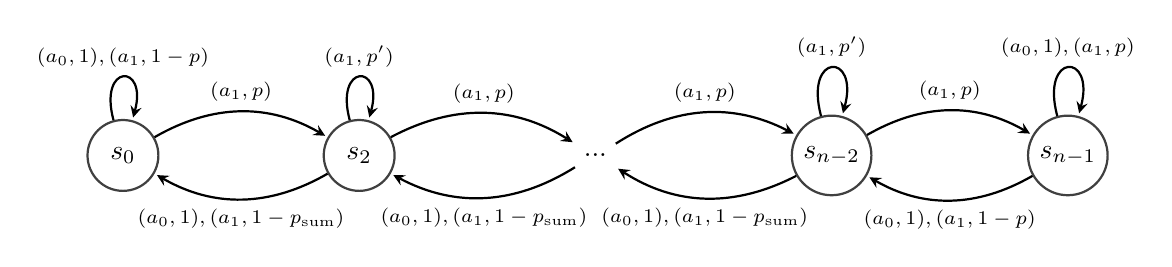
\begin{tikzpicture}[->,>=stealth,shorten >=1pt,auto,node distance=2cm,thick]
    \tikzstyle{state}=[circle,thick,draw=black!75,minimum size=9mm,inner sep=1mm]
    
    \node[state] (A) at (0,0) {$s_0$};
    \node[state] (B) at (3,0) {$s_2$};
    \node (C) at (6,0) {...};
    \node[state] (D) at (9,0) {$s_{n-2}$};
    \node[state] (E) at (12,0) {$s_{n-1}$};
    
    \path (A) edge [loop above] node[midway,above, font=\scriptsize] {$(a_0,1),(a_1,1-p)$} (A)
              edge [bend left] node[midway,above, font=\scriptsize] {$(a_1,p)$} (B)
          (B) edge [bend left] node[midway,below, font=\scriptsize] {$(a_0,1), (a_1,1-p_{\rm sum})$}  (A)
              edge [loop above] node[midway,above, font=\scriptsize] {$(a_1,p')$} (B)
              edge [bend left] node[midway,above, font=\scriptsize] {$(a_1,p)$}  (C)
          (C) edge [bend left] node[midway,below, font=\scriptsize] {$(a_0,1), (a_1,1-p_{\rm sum})$}  (B)
              edge [bend left] node[midway,above, font=\scriptsize]{$(a_1,p)$} (D)
          (D) edge [bend left] node[midway,below, font=\scriptsize] {$(a_0,1), (a_1,1-p_{\rm sum})$} (C)
              edge [loop above] node[midway,above, font=\scriptsize] {$(a_1,p')$}(D)
              edge [bend left] node[midway,above, font=\scriptsize]{$(a_1,p)$} (E)
          (E) edge [bend left] node[midway,below, font=\scriptsize] {$(a_0,1), (a_1,1-p)$}  (D)
              edge [loop above] node[midway,above, font=\scriptsize] {$(a_0,1),(a_1,p)$} (E);
    
    \end{tikzpicture}
    \caption{{\tt Riverswim} environment \cite{strehl2004empirical}. Each tuple $(a,p)$ represents the action $a$ that triggers the transition and the probability $p$ of that event.}
    \label{fig:riverswim_env}
\end{figure}
   % \draw[->] (s0) edge[bend left]  node[midway,above, font=\scriptsize] {$(a_1,0.3,\theta)$} (s1) ;


\paragraph{Forked Riverswim.} The Forked RiverSwim environment \cite{russo2023model} is a variation of the traditional RiverSwim reinforcement learning benchmark, designed to test more complex exploration strategies. In this variant, the state space branches into multiple paths, resembling a river that forks. At intermediate states the agent can switch between the forks, while the end states are not connected.  This variant requires the agent to make more sophisticated decisions to explore the environment. This setup increases the sample complexity and challenges the agent's ability to generalize across different paths within the environment.

In \cref{fig:forkedriverswim_env} is shown a depiction of the environment. There are a total of $2n+1$ states, and two parameters $p,p'\in (0,1)$,  so that $p_{\rm sum}=p+p'<1$. In the figure, each tuple $(a,p)$ represents the  action $a$ that triggers the transition and the probability $p$ of that event. The agent starts in state $s_0$, and in every state can chose between three actions $\{a_0,a_1, a_2\}$. For small values of $p$ it becomes difficult for the agent to swim right  in both forks, and larger values of $p'$ can also hinder the progress. As in Riverswim, swimming towards the left is easier, since the probability of $P(s_{i-1}|s_i, a_0)=1$. For the experiments, we used $n\in\{8,10,15\}, p=0.7, p'=6(1-p)/7$.


\begin{figure}[h]
    \centering
    \resizebox{.75\linewidth}{!}{%
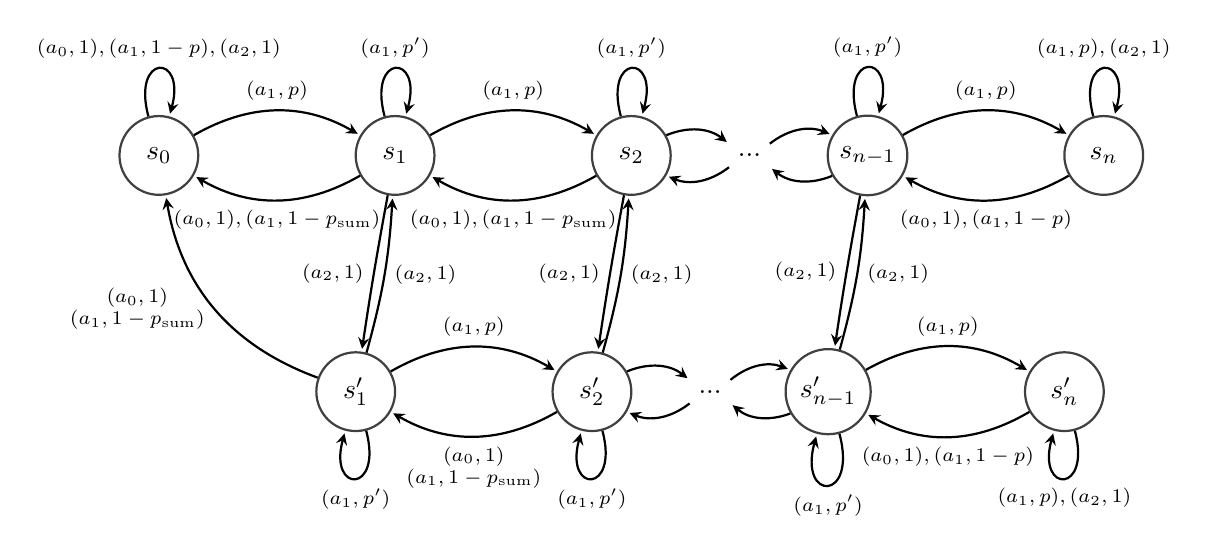
\begin{tikzpicture}[->,>=stealth,shorten >=1pt,auto,node distance=3cm,thick]
\tikzstyle{state}=[circle,thick,draw=black!75,minimum size=10mm,inner sep=1mm]

\node[state] (A) at (0,0) {$s_0$};
\node[state] (B) at (3,0) {$s_1$};
\node[state] (C) at (6,0) {$s_2$};
\node[state] (D) at (9,0) {$s_{n-1}$};
\node[state] (E) at (12,0) {$s_{n}$};
\node[state] (F) at (2.5,-3) {$s_1'$};
\node[state] (G) at (5.5,-3) {$s_2'$};
\node[state] (H) at (8.5,-3) {$s_{n-1}'$};
\node[state] (I) at (11.5,-3) {$s_{n}'$};
\node (C1) at (7.5,0) {...};
\node (C2) at (7,-3) {...};

\path (A) edge [loop above] node[midway,above, font=\scriptsize] {$(a_0,1),(a_1,1-p),(a_2,1)$} (A)
          edge [bend left] node[midway,above, font=\scriptsize] {$(a_1,p)$} (B)
          %edge [bend right=10] node[midway,below, font=\scriptsize] {0.1} (F)
      (B) edge [loop above] node[midway,above, font=\scriptsize] {$(a_1,p')$} (B)
          edge [bend left] node[midway,above, font=\scriptsize] {$(a_1,p)$} (C)
          edge [bend right=1] node[midway,left, font=\scriptsize] {$(a_2,1)$} (F)
          edge [bend left] node[midway,below, font=\scriptsize] {$(a_0,1),(a_1,1-p_{\rm sum})$}   (A)
      (C) edge [loop above] node[midway,above, font=\scriptsize] {$(a_1,p')$} (C)
          edge [bend left]  (C1)
          edge [bend right=1] node[midway,left, font=\scriptsize] {$(a_2,1)$}  (G)
          edge [bend left] node[midway,below, font=\scriptsize] {$(a_0,1),(a_1,1-p_{\rm sum})$} (B)
      (C1) edge [bend left]  (D)
           edge [bend left]  (C)
      (D) edge [loop above] node[midway,above, font=\scriptsize] {$(a_1,p')$} (D)
          edge [bend left] node[midway,above, font=\scriptsize] {$(a_1,p)$} (E)
          edge [bend left]  (C1)
          edge [bend right=1] node[midway,left, font=\scriptsize] {$(a_2,1)$} (H)
      (E) edge [loop above] node[midway,above, font=\scriptsize] {$(a_1,p),(a_2,1)$} (E)
           edge [bend left] node[midway,below, font=\scriptsize] {$(a_0,1),(a_1,1-p)$} (D)
           
      (F) edge [loop below] node[midway,below, font=\scriptsize] {$(a_1, p')$} (F)
          edge [bend left] node[midway,above, font=\scriptsize] {$(a_1,p)$} (G)
          edge [bend left=30] node[midway,left, align=center,font=\scriptsize] {$(a_0,1)$\\$(a_1,1-p_{\rm sum})$} (A)
          edge [bend right=6] node[midway,right, font=\scriptsize] {$(a_2,1)$} (B)
      (G) edge [loop below] node[midway,below, font=\scriptsize]  {$(a_1, p')$} (G)
          edge [bend left]  (C2)
          edge [bend left] node[midway,below, align=center, font=\scriptsize] {$(a_0,1)$\\$(a_1,1-p_{\rm sum})$} (F)
          edge [bend right=6] node[midway,right, font=\scriptsize] {$(a_2,1)$}  (C)
      (C2) edge [bend left]  (H)
           edge [bend left]  (G)
          
      (H) edge [loop below] node[midway,below, font=\scriptsize] {$(a_1,p')$} (H)
          edge [bend right=6] node[midway,right, font=\scriptsize] {$(a_2,1)$} (D)
          edge [bend left]  (C2)
          edge [bend left] node[midway,above, font=\scriptsize] {$(a_1,p)$} (I)
      (I) edge [loop below] node[midway,below, font=\scriptsize] {$(a_1,p),(a_2,1)$} (I)
          edge [bend left] node[midway,below, font=\scriptsize] {$(a_0,1),(a_1,1-p)$}  (H);

\end{tikzpicture}}
    \caption{{\tt Forked Riverswim} environment \cite{russo2023model}. Each tuple $(a,p)$ represents the action $a$ that triggers the transition and the probability $p$ of that event.}
    \label{fig:forkedriverswim_env}
\end{figure}


\paragraph{Double Chain.} The Double Chain environment \cite{Kaufmann21a} consists of two chains, similarly to the Forked Riverswim. The main difference consists in the fact that it is not possible to switch between the two chains, and intermediate states are transient (there is no parameter $p'$).


In \cref{fig:doublechain_env} is shown a depiction of the environment. There are a total of $2n+1$ states, and one parameters $p\in (0,1)$. In the figure, each tuple $(a,p)$ represents the  action $a$ that triggers the transition and the probability $p$ of that event. The agent starts in state $s_0$, and in every state can chose between two actions $\{a_0,a_1\}$. For small values of $p$ it becomes difficult for the agent to move to the end of the chain  in both chains. For the experiments, we used $n\in \{8,10,15\}, p=0.7$.



\begin{figure}[h]
    \centering
    \resizebox{.75\linewidth}{!}{%
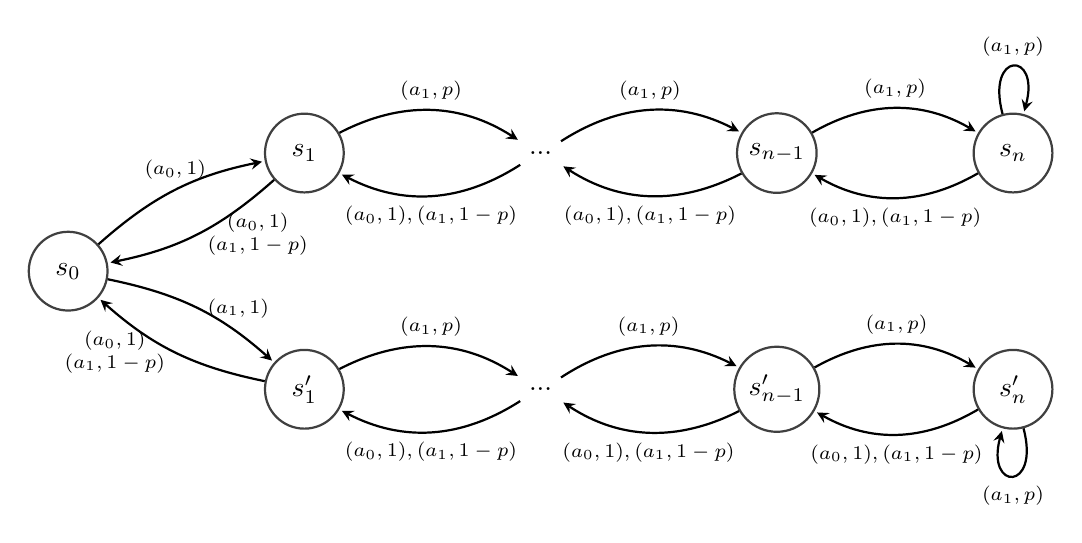
\begin{tikzpicture}[->,>=stealth,shorten >=1pt,auto,node distance=3cm,thick]
\tikzstyle{state}=[circle,thick,draw=black!75,minimum size=10mm,inner sep=1mm]

\node[state] (A) at (0,-1.5) {$s_0$};
\node[state] (B) at (3,0) {$s_1$};
\node[state] (D) at (9,0) {$s_{n-1}$};
\node[state] (E) at (12,0) {$s_{n}$};
\node[state] (F) at (3,-3) {$s_1'$};
\node[state] (H) at (9,-3) {$s_{n-1}'$};
\node[state] (I) at (12,-3) {$s_{n}'$};
\node (C1) at (6,0) {...};
\node (C2) at (6,-3) {...};

\path (A) edge [bend left=15] node[midway,above, font=\scriptsize] {$(a_0,1)$} (B)
          edge [bend left=15] node[midway,right, font=\scriptsize] {$(a_1,1)$} (F)
      (B) edge [bend left] node[midway,above, font=\scriptsize] {$(a_1,p)$} (C1)
          edge [bend left=15] node[midway,right, align=center,font=\scriptsize] {$(a_0,1)$\\$(a_1,1-p)$}   (A)

      (C1) edge [bend left]  node[midway,above, font=\scriptsize] {$(a_1,p)$}(D)
           edge [bend left] node[midway,below, font=\scriptsize] {$(a_0,1),(a_1,1-p)$}  (B)
      (D) edge [bend left] node[midway,above, font=\scriptsize] {$(a_1,p)$} (E)
          edge [bend left] node[midway,below, font=\scriptsize] {$(a_0,1),(a_1,1-p)$} (C1)
      (E) edge [loop above] node[midway,above, font=\scriptsize] {$(a_1, p)$} (E)
           edge [bend left] node[midway,below, font=\scriptsize] {$(a_0,1),(a_1,1-p)$} (D)
           
      (F) edge [bend left] node[midway,above, font=\scriptsize] {$(a_1,p)$} (C2)
          edge [bend left=15] node[midway,left, align=center,font=\scriptsize] {$(a_0,1)$\\$(a_1,1-p)$} (A)

      (C2) edge [bend left] node[midway,above, font=\scriptsize] {$(a_1,p)$} (H)
           edge [bend left] node[midway,below, font=\scriptsize] {$(a_0,1),(a_1,1-p)$} (F)
          
      (H) edge [bend left] node[midway,below, font=\scriptsize] {$(a_0,1),(a_1,1-p)$}  (C2)
          edge [bend left] node[midway,above, font=\scriptsize] {$(a_1,p)$} (I)
      (I) edge [loop below] node[midway,below, font=\scriptsize] {$(a_1,p)$} (I)
          edge [bend left] node[midway,below, font=\scriptsize] {$(a_0,1),(a_1,1-p)$}  (H);

\end{tikzpicture}
}
    \caption{{\tt Double Chain} environment \cite{Kaufmann21a} . Each tuple $(a,p)$ represents the action $a$ that triggers the transition and the probability $p$ of that event.  }
    \label{fig:doublechain_env}
\end{figure}




\paragraph{NArms.} This environment is an adaptation to $N$ arms of the original {\tt 6Arms} environment from  \cite{strehl2004empirical}. Differently from the previous environments, this is a bandit-like environment, where the agent is presented with $n$ different actions (or arms) to choose from. The agent starts in a state $s_0$ and selects an arm $a_i$. Upon selecting an arm, the agent may transition to corresponding state $s_i$. Certain arms are more difficult to observe, in the sense that the transition probability is lower. This property mimics the  probability of collecting a reward in a bandit problem.
In \cref{fig:narms_env} is shown a depiction of the environment. There are a total of $n+1$ states, and one parameters $p_0\in (0,1)$. In the figure, each tuple $(a,p)$ represents the  action $a$ that triggers the transition and the probability $p$ of that event. The notation  $a_{n_0:n_0+n}$ indicates  all the actions in $\{a_{n_0},\dots,a_{n_0+n}\}$.
The agent starts in state $s_0$, and in every state she can select between $n$ actions $\{a_0,a_1,\dots, a_{n-1}\}$. For small values of $p_0$ it becomes difficult for the agent to move to different states. Similarly, it is harder to navigate to states $s_i$ for large values of $n$. We used $p_0=0.7$ and $n\in \{10,20,30\}$.





\begin{figure}[h]
    \centering
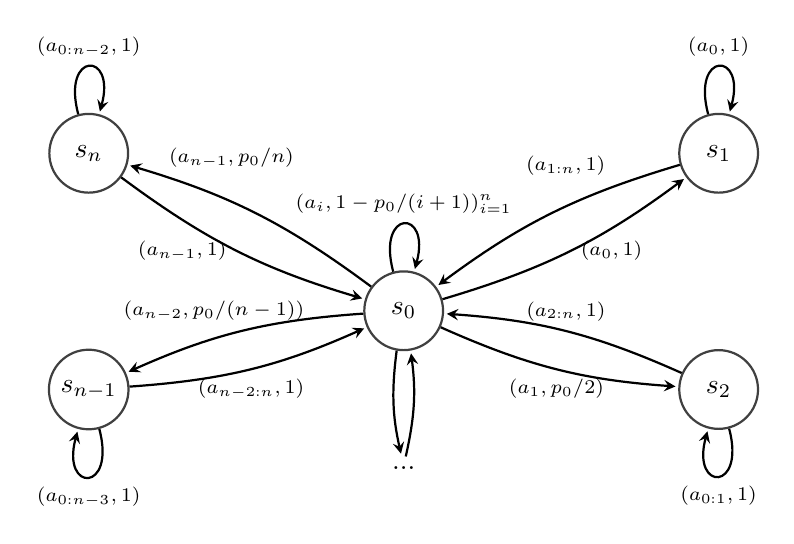
\begin{tikzpicture}[->,>=stealth,shorten >=1pt,auto,node distance=3cm,thick]
\tikzstyle{state}=[circle,thick,draw=black!75,minimum size=10mm,inner sep=1mm]

% Central hub
\node[state] (A) at (0,0) {$s_0$};

% Arms
\node[state] (B1) at (4,2) {$s_1$};
\node[state] (B2) at (4,-1) {$s_2$};
\node  (C) at (0,-2) {...};
\node[state] (B5) at (-4,2) {$s_n$};
\node[state] (B6) at (-4,-1) {$s_{n-1}$};

\path (A) edge [bend right=10] node[midway,right, font=\scriptsize] {$(a_0,1)$} (B1)
          edge [bend right=10] node[midway,below, font=\scriptsize] {$(a_1,p_0/2)$} (B2)
          edge [bend right=10] (C)
          edge [bend right=10] node[midway,right, font=\scriptsize,yshift=20pt,xshift=-35pt] {$(a_{n-1}, p_0/n)$} (B5)
          edge [bend right=10] node[midway,above, font=\scriptsize, xshift=-10pt] {$(a_{n-2}, p_0/(n-1))$} (B6)
          edge [loop above] node[midway,above, font=\scriptsize] {$(a_i, 1- p_0/(i+1))_{i=1}^n$} (A)
      (B1) edge [bend right=10] node[midway,above, font=\scriptsize,yshift=10pt,xshift=5pt] {$(a_{1:n},1)$} (A)
           edge [loop above] node[midway,above, font=\scriptsize] {$(a_{0},1)$} (B1)
      (B2) edge [bend right=10] node[midway,above, font=\scriptsize] {$(a_{2:n},1)$} (A)
           edge [loop below] node[midway,below, font=\scriptsize] {$(a_{0:1},1)$} (B2)

      (C) edge [bend right=10] node[midway,below, font=\scriptsize] {} (A)

      (B5) edge [bend right=10] node[midway,left, font=\scriptsize] {$(a_{n-1},1)$} (A)
       edge [loop above] node[midway,above, font=\scriptsize] {$(a_{0:n-2},1)$} (B5)
      (B6)  edge [bend right=10] node[midway,below, font=\scriptsize] {$(a_{n-2:n},1)$} (A)
      edge [loop below] node[midway,below, font=\scriptsize] {$(a_{0:n-3},1)$} (B6);

\end{tikzpicture}

    \caption{{\tt NArms} environment. Each tuple $(a,p)$ represents the action $a$ that triggers the transition and the probability $p$ of that event. In the figure the notation $a_{n_0:n_0+n}$ indicates  all the actions in $\{a_{n_0},\dots,a_{n_0+n}\}$. In state $s_0$ the probability to remain in $s_0$ for any action $a_i$ is $P(s_0|s_0,a_i)=1-p_0/(i+1)$, with the exception that $P(s_0|s_0,a_0)=0$.}
    \label{fig:narms_env}
\end{figure}



\subsection{Algorithm Details}\label{app:algorithms}
In this section we briefly explain the mechanisms of each algorithm used in the experiments, and, in case, their adaptation. Note that for all algorithms we evaluated the policies by  using the MDP estimate $M_t$ through policy evaluation.


\paragraph{ Noisy Policy (Uniform).} This method simply computes a mixture of the target policies $\pi_{\rm mix}(a|s) = \frac{|\{\pi\in \Pi: \pi(s)=a\}|}{|\Pi|}$, which is then mixed with a uniform policy $\pi_u$ with a constant mixing factor $\varepsilon_t=0.3$. The resulting behavior policy is $\pi_b =(1-\varepsilon_t)\pi_{\rm mix} +\varepsilon_t \pi_u$.

\paragraph{Noisy Policy (Visitation).} This method is similar to the previous one, but the mixing factor is not constant anymore. We take a mixing factor that is $\epsilon_t=1/N_t(s_t)$, which based on the number of visits to state $s_t$. The resulting behavior policy is $\pi_b =(1-\varepsilon_t)\pi_{\rm mix} +\varepsilon_t \pi_u$.

\paragraph{SF-NR \cite{mcleod2021continual}.} This is an algorithm for multi-task policy evaluation based on the Successor Representation. The pseudo-steps of the algorithm can be found in \cref{algo:sfnr}. The method maintains a successor representation $\psi_{\pi,t}$ for each policy $\pi$, as well as a behavior policy $\pi_\beta$. These are learned using TD-learning, and the behavior policy uses the variation between $\psi_{\beta,t+1}$ and $\psi_{\beta,t}$ as a reward. 
In our experiment we used a temperature $T=2$ and a discount factor for the successor representation $\gamma_\psi=0.99$.

\begin{algorithm}[h]
	\caption{{\tt SF-NR}}
	\label{algo:sfnr}
    \small
	\begin{algorithmic}[1]
    \REQUIRE Discount factor $\gamma$; Temperature $T$; Successor discount factor $\gamma_\psi$; policy set $\Pi$.
    \STATE Set $\pi_\beta(\cdot|s)={\cal U}(\{1,\dots,A\})$ for all states $s$.
    \STATE Set $\psi_{\pi,1}(s,a)=1$ for all $(s,a)$.
    \WHILE{not done} 
            \STATE Compute $\hat \pi_\beta(\cdot|s_t) = {\tt Softmax}(\pi_\beta(\cdot|s_t)/T)$
            \STATE Sample $a_t$ from $(1-\varepsilon_t)\hat \pi_\beta(\cdot|s_t)  +\varepsilon_t/A$ and observe $s_{t+1}\sim P(\cdot|s_t,a_t)$.
            \FOR{$\pi \in \Pi$}
                \STATE Compute $\delta_t=1+\gamma_\psi \psi_{\pi,t}(s_{t+1},\pi(s_{t+1}))-\psi_{\pi,t}(s_t,a_t)$
                \STATE Set $\psi_{\pi,t+1}(s_t,a_t)= \psi_{\pi,t}(s_t,a_t) + \alpha_t \delta_t$, where $\alpha_t=1/N_t(s_t,a_t)$.
            \ENDFOR
            \STATE Compute $\delta_{\psi,t}=1/|\Pi| \sum_{\pi\in \Pi}\|{\rm Vec}(\psi_{\pi,t+1})- {\rm Vec}(\psi_{\pi,t})\|_1$.
            \STATE Update $\pi_\beta(a_t|s_t)\gets \pi_\beta(a_t|s_t)+ \alpha_t\left(\delta_{\psi,t}+ \gamma \max_a\pi_\beta(a|s_{t+1}) - \pi_\beta(a_t|s_t)\right)$, where $\alpha_t=1/N_t(s_t,a_t)$.
            \STATE Update MDP estimate $M_t$ and set $t\gets t+1$.
            \ENDWHILE{}
	\end{algorithmic}
\end{algorithm}



\paragraph{GVFExplorer \cite{jain2024adaptive}.}  This method considers variance-based exploration strategy for learning general value functions \cite{sutton2011horde} based on minimizing the MSE. 
 The pseudo-steps of the algorithm can be found in \cref{algo:gvf}. 
Given the current estimate of the MDP $M_t$, the method estimates ${\rm Var}_{s,a}^\pi(t)$, the variance of the return $G^\pi=r_1+\gamma r_2+\gamma^2 r_3+\dots$ under $\pi$ staring from $(s,a)$, $\forall\pi\in \Pi, (s,a)\in \statespace\times\actionspace$. Then, a behavior policy is computed as $
\pi_\beta(a|s) = \frac{\sqrt{\sum_{\pi\in\Pi} \pi(a|s)  {\rm Var}_{s,a}^\pi(t)}}{\sum_b\sqrt{\sum_{\pi\in\Pi} \pi(b|s)  {\rm Var}_{s,b}^\pi(t)}}$. Lastly, we mix this policy with a uniform policy. For this method we used a fixed mixing factor $\varepsilon=0.3$ (we did not use a visitation based mixing factor because performance deteriorated).





\begin{algorithm}[h]
	\caption{{\tt GVFExplorer}}
	\label{algo:gvf}
    \small
	\begin{algorithmic}[1]
    \REQUIRE Mixing factor $\varepsilon$, policy set $\Pi$.
    \STATE Set ${\rm Var}_{s,a}^\pi(1)=1$ for all $(s,a)\in \statespace\times\actionspace, \pi\in \Pi$.
    \WHILE{not done} 
            \STATE Set $\pi_\beta(a|s) = \frac{\sqrt{\sum_{\pi\in\Pi} \pi(a|s)  {\rm Var}_{s,a}^\pi(t)}}{\sum_b\sqrt{\sum_{\pi\in\Pi} \pi(b|s)  \rm Var_{s,b}^\pi(t)}}$
            \STATE Sample $a_t$ from $(1-\varepsilon) \pi_\beta(\cdot|s_t)  +\varepsilon/A$ and observe $s_{t+1}\sim P(\cdot|s_t,a_t)$.
            \STATE Update MDP estimate $M_t$, variance estimates $\{{\rm Var}^\pi(t)\}_{\pi\in \Pi}$ and set $t\gets t+1$.
            \ENDWHILE{}
	\end{algorithmic}
\end{algorithm}
Note that $\pi_\beta$ is similar to the generative solution in \cref{eq:T_epsilon_omega} (i.e., $\Omega(M)=\Delta(\statespace\times\actionspace)$). In fact, {\tt GVFExplorer}  neglects the forward equations when deriving $\pi_\beta$. The resulting solution does not take into account the dynamics induced by the behavior policy, effectively making it a generative method (compare with the generative solution proved in \cite{al2021adaptive,russo2023model}). We believe this is due to a term being omitted  in the proof of \citet[Theorem 4.1]{jain2024adaptive}  that accounts for how changes in the state distribution induced by the behavior policy impact the variance. 
  

\paragraph{MR-NaS.} For \mrnas{} we computed the exploration strategy $\omega_t^\star$ every $500$ steps in the environment, to avoid excessive computational burden.
The policy is then mixed with a forcing policy that is $\pi_{f,t}(\cdot|s)=\texttt{softmax}\left(-\beta_t(s) N_t(s,\cdot)\right)$
with $\beta_t(s) = \frac{\beta  \log(N_t(s))}{\max_a |N_t(s,a) - \min_b N_t(s,b)|}, \beta\in [0,1]$ and  $({\tt softmax}(x))_i=e^{x_i}/\sum_j e^{x_j}$ for a vector $x$. This choice encourages to select under-sampled actions for $\beta > 0$, while for $\beta=0$ we obtain a uniform forcing policy $\pi_{f,t}(a|s)=1/A$. 
 We then mix $\omega_t^\star$ with $\pi_{f,t}$ using a mixing factor $\epsilon_t = 1/\max(1,N_t(s_t))^\alpha$, with $N_t(s) = \sum_a N_t(s,a)$. The values $\alpha,\beta$ need to guarantee $\alpha+\beta\leq 1$ \cite{russomulti}, hence we chose $\alpha=0.99$ and $\beta=0.01$.

\subsection{Additional Results}\label{app:additional_results}
In this sub-section we report additional  results. To run reproduce the results, we refer the reader to the {\tt README.md} file in the supplementary material. In \cref{fig:app:multi_pol_multi_rew} are reported the results for the multi-reward multi-policy case with various sizes of the state space. Similarly, in \cref{fig:app:rew_free_multi_pol} are reported the reward-free results for the multi-policy case, and in \cref{fig:app:single_pol_rewfree} the results for the single-policy reward-free case. Experiments were run over $10^6$ time-steps, with $30$ seeds. Confidence intervals were computed using bootstrap \cite{efron1992bootstrap}.

\begin{figure}
    \centering
    \includegraphics[width=\linewidth]{figures/1000000_multi_policy_multi_reward_abs_error_small.pdf}
    \includegraphics[width=\linewidth]{figures/1000000_multi_policy_multi_reward_abs_error_medium.pdf}
    \includegraphics[width=\linewidth]{figures/1000000_multi_policy_multi_reward_abs_error_large.pdf}
    \caption{Multi-reward multi-policy evaluation for different sizes of the MDPs: from top to bottom the state space size is $15, 20, 30$. Shaded curves represent 95\% confidence intervals.}
    \label{fig:app:multi_pol_multi_rew}
\end{figure}

\begin{figure}
    \centering
    \includegraphics[width=\linewidth]{figures/1000000_multi_policy_rewfree_abs_error_small.pdf}
    \includegraphics[width=\linewidth]{figures/1000000_multi_policy_rewfree_abs_error_medium.pdf}
    \includegraphics[width=\linewidth]{figures/1000000_multi_policy_rewfree_abs_error_large.pdf}
    \caption{Reward-Free multi-policy evaluation for different sizes of the MDPs: from top to bottom the state space size is $15, 20, 30$. Here we depict the average error over the canonical basis  ${\cal R}_{\rm canonical}$. Shaded curves represent 95\% confidence intervals.}
    \label{fig:app:rew_free_multi_pol}
\end{figure}

\begin{figure}
    \centering
    \includegraphics[width=\linewidth]{figures/1000000_single_policy_rewfree_abs_error_small.pdf}
    \includegraphics[width=\linewidth]{figures/1000000_single_policy_rewfree_abs_error_smedium.pdf}
    \includegraphics[width=\linewidth]{figures/1000000_single_policy_rewfree_abs_error_large.pdf}
    \caption{Reward-Free single-policy evaluation for different sizes of the MDPs: from top to bottom the state space size is $15, 20, 30$. Here we depict the average error over the canonical basis  ${\cal R}_{\rm canonical}$. Shaded curves represent 95\% confidence intervals.}
    \label{fig:app:single_pol_rewfree}
\end{figure}